\chapter{Bevezető}

\section{Feladat háttere}

Egyre több szöveges tartalom születik az interneten, ezért aki arra vállalkozik, hogy ezekből manuálisan információt nyerjen ki, egyre nehezebb problémával találja szembe magát. Az én feladatom egy olyan rendszer fejlesztése, amely automatizált módon képes számos információ-kinyeréssel kapcsolatos feladat ellátására.

\section{Célok}

Célom egy olyan információkinyerő rendszer fejlesztése volt, ami képes számos monoton feladat ellátására, mint például a szövegklasszifikáció, kulcsszó- és entitásfelismerés, valamint a szöveg kontextusában rejlő entitások közti kapcsolatra utaló információ kinyerése. A rendszer lényeges részét képezi egy webes felület, amely lehetőséget biztosít a felhasználóknak a szoftver által végzett döntések ellenőrzésére és javítására.

A feladatot internetről származó hírek szövegén szerettem volna megoldani, ezért ilyen adatok gyűjtésére és tisztítására is szükség volt. Az összeállított korpusz segítségével akartam olyan modelleket tanítani, amik megoldanak emberek számára időigényes feladatokat, legalább olyan pontossággal, hogy az később segítséget jelentsen.

A rendszer fejlesztése során különös figyelmet fordítottam arra, hogy az legyen képes a legújabb nyelvtechnológiai megoldások - mint például a nagy nyelvi modellek - integrálására. Ez amellett, hogy lehetőséget biztosít eddig nehezen megoldható feladatok támogatására, új nehézségeket is felvet az erőforrásigény kapcsán.

A célkitűzések között szerepelt továbbá teljesítménymértékek meghatározása, hogy objektíven értékelhető legyen a rendszer pontossága. Ez magában foglalta különböző pontosságot mutató kísérletek végrehajtását és a rendszer egyes komponenseinek futási idejének mérését.

\section{Részfeladatok}

\subsection{Klasszifikáció}

%Mivel a feladat korrupcióval kapcsolatos cikkek szövegével kapcsolatos, első lépésként fontos megállapítani az egyes cikkekről, hogy ilyen témát dolgoznak-e fel, ebben segít a szövegklasszifikáció. Ez egy szövegelemzési eljárás, ami gépi tanulás segítségével képes egy adott szöveget osztályokba sorolni. Aszerint, hogy hány lehetséges osztály közül kell választani megkülönböztetünk bináris (két osztály) és multi-label (kettőnél több osztály) klasszifikációt. Jelen esetben a feladat csak azt követeli meg, hogy az adott szövegről eldöntsük beleillik-e egy konkrét témába, így elegendő a bináris klasszifikáció alkalmazása.

Mivel a feladat nem általános, hanem témaspecifikus újságcikkek szövegével kapcsolatos, első lépésként fontos megállapítani az egyes cikkekről, hogy olyan témát dolgoznak-e fel, ami a feladat szempontjából érdekes, ebben segít a szövegklasszifikáció. Ez egy szövegelemzési eljárás, ami gépi tanulás segítségével képes egy adott szöveget osztályokba sorolni. Aszerint, hogy hány lehetséges osztály közül kell választani megkülönböztetünk bináris (két osztály) és multi-label (kettőnél több osztály) klasszifikációt. Jelen esetben a feladat csak azt követeli meg, hogy az adott szövegről eldöntsük beleillik-e egy konkrét témába, így elegendő a bináris klasszifikáció alkalmazása.

A klasszifikáció kimenete azonban nem csak osztály lehet, sok módszer lehetőséget nyújt arra is, hogy az egyes osztályok modell által vélt valószínűségét is elárulja. Ez a kiegészítő információ felhasználható arra, hogy a klasszifikáció eredményét hangoljuk azzal, hogy pozitív eredmény esetén 50\%-nál nagyobb valószínűséget követelünk meg az elfogadáshoz, vagy épp fordítva.

% masik cikk hianyzik
\subsection{Névelemfelismerés és -klasszifikáció}

Az információkinyerés során egy kifejezetten fontos lépés a névelemfelismerés (Named Entity Recognition). Ez a szövegben előforduló entitások (például: személyek, intézmények, helyszínek) kinyerése és ellátása egy típusára utaló címkével.

Ez a folyamat csupán szövegrészleteket azonosít és adja meg az ott talált névelem típusát, így könnyen előfordulhat, hogy a felismert szövegrész nem egy teljes név, hanem annak csupán egy része: kereszt- vagy vezetéknév.

Az adatbázis bővítése szempontjából nem elegendő a névelemeket azonosítani, azokat még tovább kell szűrni a relevanci alapján, ami egy névelem klasszifikációs feladat. Emellett ebben a részfeladatban csökkentem a névelemek listáját a teljes nevekre.

\subsection{Kulcsszavak kinyerése}

A kulcsszókinyerés alatt általában a szövegben előforduló szavak frekvencia alapján való kiválasztását szokták érteni (például TF-IDF módszer). Azonban előfordulhat ennél tágabb definíciója a kulcsszónak, amikor nem feltétlenül szerepel az adott kulcsszó a szövegben és helyette egy előre meghatározott listából kell kiválasztani.

Ha a lehetséges kulcsszavak listája előre ismert ez a kulcsszókinyerés értelmezhető egy nagyon sok osztályos szöveg-klasszifikációs feladatként is.

\subsection{Névelemek közti kapcsolat kinyerése}

A korábbi lépésben megszerzett személyek és intézmények közötti összefüggések névelem-névelem-kapcsolat hármasokkénti kinyerése is cél. A névelem esetében fontos, hogy a teljes nevet tartalmazza, a kapcsolat viszont szabad szöveg. Ezen kapcsolatok kinyerése magában hordozza a tévedés lehetőségét, ezért segít, ha szövegkörnyezetet is csatolunk melléjük. Emellett manapság a generatív nagy nyelvi modellek már arra is lehetőséget adnak, hogy egy indoklást is rendeljünk a kinyert hármashoz.

\begin{figure}[H]
	\centering
	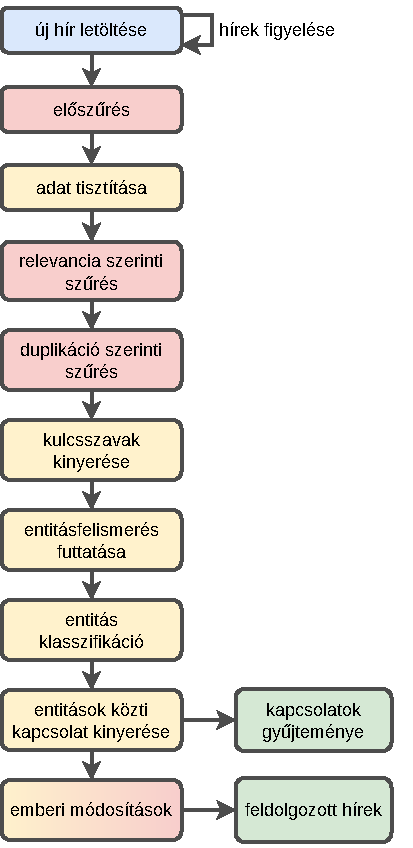
\includegraphics[width=100mm,keepaspectratio]{figures/flowchart.pdf}
	\caption{Rendszer működését bemutató folyamatábra}
\end{figure}
